\documentclass[beamer]{standalone}
\usepackage[T1]{fontenc}
\usepackage[utf8]{inputenc}
\usepackage[english]{babel}
\usepackage{csquotes}

\usepackage[
    style=alphabetic,
    backend=biber,
 ]{biblatex}
\bibliography{../references}

\usepackage{tikz}

\usetikzlibrary{backgrounds}
\usetikzlibrary{positioning}

\definecolor{almost-white}{HTML}{fefefe}


\begin{document}

\begin{standaloneframe}


\begin{tikzpicture}[%
    background rectangle/.style={ draw=almost-white, line width=0pt, },
    show background rectangle,
]


\only<1-2>{
    \draw [->,-latex] (0,0) to (10,0);
}

\only<3->{
    \draw (0,0) to (1.25,0);
    \draw [dashed] (1.25,0) to (4,0);
    \draw [->,-latex] (4,0) to (10,0);
}


\onslide<2->
\draw (.75,.25) node [above] {1976} to ++(0,-.5) node [below] {\textbf<2>{\cite{Val76}}};

\onslide<4->
\draw (4.5,.25) node [above] {2008} to ++(0,-.5) node [below] {\textbf<4>{\cite{KS08}}};

\onslide<5>
\draw (7.75,.25) node [above] {2016} to ++(0,-.5) node [below, text width=2cm, align=center] {\textbf<5>{\cite{KS16}} \\ \phantom{\cite{LMS16}}};

\onslide<6->
\draw (7.75,.25) node [above] {2016} to ++(0,-.5) node [below, text width=2cm, align=center] {\textbf<8>{\cite{KS16}} \\ \textbf<6>{\cite{LMS16}}};

\onslide<7->
\draw (9.25,.25) node [above] (y17) {2017} to ++(0,-.5) node [below] {\textbf{\cite{GKS17}}};

% hack
\node [inner sep=0, above=0 of y17] {};

\end{tikzpicture}

\end{standaloneframe}

\end{document}
